%!TEX root = Handbuch.tex

\section{Speicherstruktur}

\subsection{Das .emp-Verzeichnis}
Beim Benutzen des \textbf{init}-Befehls wird im aktuellen Vezeichnis ein .emp-Ordner erstellt. Dieser dient sowohl zu Identifizierung der Repository-Wurzel, als auch zum speichern sämmtlicher Schlüssel-Typ-Deklarationen.
Die im .emp-Ordner enthaltenen Dateien symbolisieren dabei einfache Variablen und enthalten nur den Typ, Ordner dagegen symbolisieren Collections und enthalten eine Sammlung der eben genannten Dateien.

\subsection{Vererbung von Werten}
Durch die Vererbung von Attributen können Wiederholungen von Eingaben von häufig auftretenden Daten eingespart werden.

Ein Wert behält in allen Unterverzeichnissen seine Gültigkeit, in denen er nicht durch Neudefinition überschrieben wurde. Dadurch können wiederkehrende Daten, wie beispielsweise die eigene Anschrift, effizient gespeichert werden. Sollte in einer Ausnahme dieser Regelung doch ein anderer Wert benötigt werden kann dieser einfach im entsprechend gewünschten Verzeichnisbaum überschrieben werden.

Hierzu ein kleines Beispiel (TODO: iwie ordentlicher machen...):


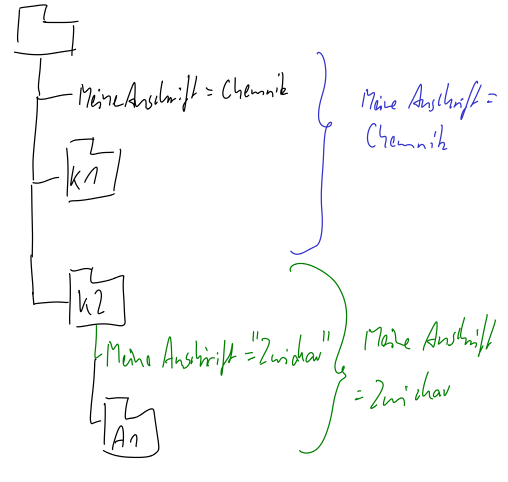
\includegraphics[width=0.8\textwidth]{04-ordnerstruct.png}

